\documentclass[12pt, a4paper]{ctexart}
\usepackage{amsmath, amsthm, amssymb, bm, color, framed, graphicx, hyperref, mathrsfs}
\usepackage{graphicx,subfigure}
\linespread{1.5}
\newenvironment{problem}{\par\noindent\textbf{习题}}{\par}
\newenvironment{solution}{\par\noindent\textbf{解答. }}{\par}
\newenvironment{note}{\par\noindent\textbf{题目\arabic{problemname}的注记. }}{\par}
\begin{document}
\title{\textbf{理论力学课后习题答案}}
\author{动力学习部}
\date{\today}
\maketitle
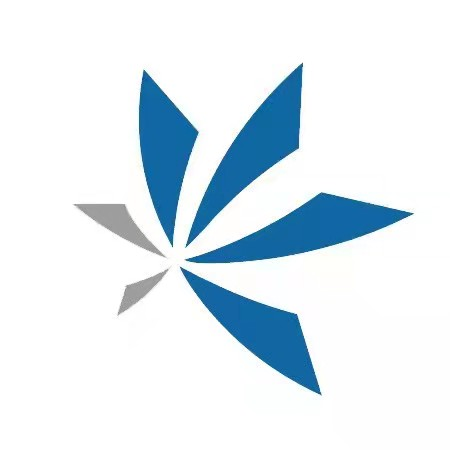
\includegraphics[scale=0.8]{2.jpg}
\newpage
\pagenumbering{roman}
\tableofcontents
\newpage
\pagenumbering{arabic}
\section{第五章习题答案}
\begin{problem}[5.18]
图示半径为$R$的圆盘以匀角速度$\omega_1$绕水平轴$ CD $转动,此轴又以匀角速度$\omega_2 $绕铅垂轴转动。试求圆盘上1点和2点的速度和加速度。
\end{problem}

\begin{figure}[ht]
	\centering
	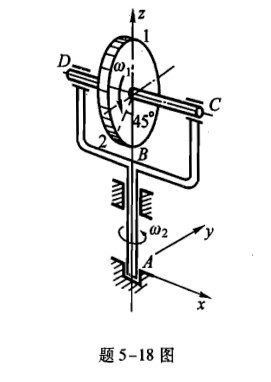
\includegraphics[scale=0.7]{3.jpg}
\end{figure}

\begin{solution}
	已1点为动点,$CD$轴为动系,$A$点为定系,由题意,则有
	\[
		\vec{v_{a_{1}}}=\vec{v_{e_1}}+\vec{v_{r_1}} \quad \vec{v_{e_1}}=0
	\]
	$\therefore \vec{v_{a_1}}=\vec{v_{r_1}}=\omega \cdot R$  
\end{solution}
\end{document}